\documentclass[oneside,a4paper,14pt]{extarticle}
\usepackage[T1,T2A]{fontenc}
\usepackage[
a4paper,
letterpaper,
top=2cm,
bottom=2cm,
left=2.5cm,
right=1.5cm
]{geometry}
\usepackage[utf8]{inputenc}
\usepackage[russian]{babel}
\usepackage{textcomp}
\usepackage{indentfirst}
\usepackage{listings}
\usepackage{xcolor}
\usepackage{enumitem}
\usepackage{graphicx}
\usepackage{mwe}
\usepackage{wrapfig}
\usepackage{caption}
\usepackage{amsmath}
\usepackage{amsfonts}
\usepackage{float}
\usepackage{amsthm}
\usepackage[all]{xy}
\usepackage[breaklinks]{hyperref}
\usepackage{titlesec}
\usepackage{adjustbox}
\usepackage{tikz}
\usetikzlibrary{positioning,arrows.meta,shapes.multipart}

\titleformat{\section}
{\normalsize\bfseries}
{\thesection} {1em}{}
\titleformat{\subsection}
{\normalsize\bfseries}
{\thesubsection} {1em}{}
\titleformat{\subsubsection}
{\normalsize\bfseries}
{\thesubsubsection} {1em}{}
\renewcommand\baselinestretch{1.33}
\normalsize
\setlength{\parindent}{1.25cm}

\lstset{
	language=Python,
	basicstyle=\ttfamily\small,
	keywordstyle=\color{blue},
	commentstyle=\color{green!60!black},
	stringstyle=\color{red},
	numbers=left,
	numberstyle=\tiny\color{gray},
	frame=single,
	breaklines=true,
	showstringspaces=false,
	tabsize=4,
	inputencoding=utf8,
	extendedchars=true,
	literate={а}{{\selectfont\char224}}1 {б}{{\selectfont\char225}}1 {в}{{\selectfont\char226}}1 {г}{{\selectfont\char227}}1 {д}{{\selectfont\char228}}1 {е}{{\selectfont\char229}}1 {ё}{{\"e}}1 {ж}{{\selectfont\char230}}1 {з}{{\selectfont\char231}}1 {и}{{\selectfont\char232}}1 {й}{{\selectfont\char233}}1 {к}{{\selectfont\char234}}1 {л}{{\selectfont\char235}}1 {м}{{\selectfont\char236}}1 {н}{{\selectfont\char237}}1 {о}{{\selectfont\char238}}1 {п}{{\selectfont\char239}}1 {р}{{\selectfont\char240}}1 {с}{{\selectfont\char241}}1 {т}{{\selectfont\char242}}1 {у}{{\selectfont\char243}}1 {ф}{{\selectfont\char244}}1 {х}{{\selectfont\char245}}1 {ц}{{\selectfont\char246}}1 {ч}{{\selectfont\char247}}1 {ш}{{\selectfont\char248}}1 {щ}{{\selectfont\char249}}1 {ъ}{{\selectfont\char250}}1 {ы}{{\selectfont\char251}}1 {ь}{{\selectfont\char252}}1 {э}{{\selectfont\char253}}1 {ю}{{\selectfont\char254}}1 {я}{{\selectfont\char255}}1 {А}{{\selectfont\char192}}1 {Б}{{\selectfont\char193}}1 {В}{{\selectfont\char194}}1 {Г}{{\selectfont\char195}}1 {Д}{{\selectfont\char196}}1 {Е}{{\selectfont\char197}}1 {Ё}{{\"E}}1 {Ж}{{\selectfont\char198}}1 {З}{{\selectfont\char199}}1 {И}{{\selectfont\char200}}1 {Й}{{\selectfont\char201}}1 {К}{{\selectfont\char202}}1 {Л}{{\selectfont\char203}}1 {М}{{\selectfont\char204}}1 {Н}{{\selectfont\char205}}1 {О}{{\selectfont\char206}}1 {П}{{\selectfont\char207}}1 {Р}{{\selectfont\char208}}1 {С}{{\selectfont\char209}}1 {Т}{{\selectfont\char210}}1 {У}{{\selectfont\char211}}1 {Ф}{{\selectfont\char212}}1 {Х}{{\selectfont\char213}}1 {Ц}{{\selectfont\char214}}1 {Ч}{{\selectfont\char215}}1 {Ш}{{\selectfont\char216}}1 {Щ}{{\selectfont\char217}}1 {Ъ}{{\selectfont\char218}}1 {Ы}{{\selectfont\char219}}1 {Ь}{{\selectfont\char220}}1 {Э}{{\selectfont\char221}}1 {Ю}{{\selectfont\char222}}1 {Я}{{\selectfont\char223}}1 {«}{{\guillemotleft}}1 {»}{{\guillemotright}}1 {№}{{\textnumero}}1 {–}{{--}}1,
}

\begin{document}
	\sloppy
	\newpage\thispagestyle{empty}
	\begin{center}
		МИНИСТЕРСТВО НАУКИ И ВЫСШЕГО ОБРАЗОВАНИЯ\\
		РОССИЙСКОЙ ФЕДЕРАЦИИ\\
		ФЕДЕРАЛЬНОЕ ГОСУДАРСТВЕННОЕ БЮДЖЕТНОЕ\\
		ОБРАЗОВАТЕЛЬНОЕ УЧРЕЖДЕНИЕ ВЫСШЕГО ОБРАЗОВАНИЯ\\
		<<ВЯТСКИЙ ГОСУДАРСТВЕННЫЙ УНИВЕРСИТЕТ>>\\
		Институт математики и информационных систем\\
		Факультет автоматики и вычислительной техники\\
		Кафедра электронных вычислительных машин
	\end{center}
	\vspace{20mm}
	\begin{center}
		Отчёт по лабораторной работе №5\\
		по дисциплине\\
		<<Базы данных>>\\
	\end{center}
	\vspace{48mm}
	\noindent
	Выполнил студент гр. ИВТб-2303-06-00 \hfill \rule[-0,5mm]{30mm}{0.15mm}\,/Шубин В. Ю./
	\newline
	Проверил преподаватель кафедры ЭВМ \hfill \rule[-0,5mm]{30mm}{0.15mm}\,/Клюкин В. Л./
	\vfill
	\begin{center}
		Киров\\
		2026
	\end{center}
	\newpage
	\thispagestyle{empty}
	\section*{Цель работы:} Познакомиться с библиотекой в языке Python для связывания приложения с базой данных, освоить на практике основы взаимодействия с БД под управлением PostgreSQL в приложении на Python с графическим интерфейсом.
	
	\section*{Среда разработки:} PostgreSQL 18, pgAdmin 4, Python 3.12 (Tkinter, tkcalendar, psycopg2), Windows 10.
	
	\newpage
	
	\section*{1. Архитектура приложения и диаграмма классов}
	
	Для выполнения работы использована таблица \texttt{review} («Отзывы на видеоигры») схемы \texttt{lab\_schema} базы данных \texttt{lab\_db}, содержащая внешний ключ \texttt{game\_id} на родительскую таблицу \texttt{game} («Видеоигры»), числовое поле оценки \texttt{score} и поле даты \texttt{review\_date}.
	
	В соответствии с методическими указаниями и шаблоном проектирования \textbf{Repository (DAO)} приложение разделено на следующие классы:
	\begin{itemize}
		\item \texttt{Database} (\texttt{database.py}) --- класс управления подключением к СУБД PostgreSQL (\texttt{openConnection}, \texttt{closeConnection}) и выполнения запросов и транзакций (\texttt{query}, \texttt{execute\_scalar});
		\item \texttt{GameItem} и \texttt{Review} (\texttt{models.py}) --- классы сущностей предметной области (Domain Model);
		\item \texttt{GameRepository} (\texttt{repositories.py}) --- репозиторий для получения списка игр из родительской таблицы \texttt{game};
		\item \texttt{ReviewRepository} (\texttt{repositories.py}) --- репозиторий для чтения отзывов, регистронезависимой фильтрации через SQL-запрос, проверки дубликатов, а также сохранения и удаления строк через функции PL/pgSQL;
		\item \texttt{ReviewApp} (\texttt{main.py}) --- класс главного окна графического интерфейса на базе \texttt{tkinter}, \texttt{ttk} и календаря \texttt{tkcalendar.DateEntry}.
	\end{itemize}
	
	Диаграмма классов, организующих работу с БД, представлена на рисунке~1.
	
	\begin{figure}[H]
		\centering
		\begin{adjustbox}{max width=\linewidth}
		\begin{tikzpicture}[
			classbox/.style={
				rectangle split,
				rectangle split parts=3,
				draw=black,
				thick,
				fill=white,
				font=\ttfamily\scriptsize,
				align=left,
				inner sep=6pt
			},
			rel/.style={-{Stealth[length=3mm, width=2.2mm]}, thick},
			dep/.style={-{Stealth[length=3mm, width=2.2mm]}, thick, dashed}
		]
			% Top: ReviewApp
			\node[classbox, text width=8.8cm] (app) at (0, 0) {
				\textbf{\centerline{ReviewApp (tk.Tk)}}
				\nodepart{second}
				- \_game\_repo : GameRepository\\
				- \_review\_repo : ReviewRepository\\
				- \_games\_map : dict[str, int]\\
				- \_current\_review\_id : Optional[int]
				\nodepart{third}
				+ load\_games() : None\\
				+ load\_reviews(filter\_pattern : str) : None\\
				+ validate\_input() : Optional[tuple]\\
				+ on\_add() : None\\
				+ on\_update() : None\\
				+ on\_delete() : None\\
				+ on\_filter() : None\\
				+ on\_numeric\_keypress(event) : str
			};

			% Middle: Repositories
			\node[classbox, text width=7.2cm] (gameRepo) at (-5.2, -5.8) {
				\textbf{\centerline{GameRepository}}
				\nodepart{second}
				- \_db : Database
				\nodepart{third}
				+ \_\_init\_\_(db : Database)\\
				+ get\_all() : List[GameItem]
			};

			\node[classbox, text width=8.4cm] (revRepo) at (5.0, -6.5) {
				\textbf{\centerline{ReviewRepository}}
				\nodepart{second}
				- \_db : Database
				\nodepart{third}
				+ \_\_init\_\_(db : Database)\\
				+ get\_all() : List[Review]\\
				+ filter\_by\_reviewer(pattern : str) : List[Review]\\
				+ exists(game\_id : int, reviewer : str, exclude\_id : int) : bool\\
				+ save(review : Review) : int\\
				+ delete(review\_id : int) : None
			};

			% Bottom row: GameItem, Database, Review
			\node[classbox, text width=5.0cm] (gameItem) at (-6.8, -12.3) {
				\textbf{\centerline{GameItem}}
				\nodepart{second}
				+ id : int\\
				+ title : str
				\nodepart{third}
				+ \_\_str\_\_() : str
			};

			\node[classbox, text width=6.0cm] (db) at (0.0, -12.3) {
				\textbf{\centerline{Database}}
				\nodepart{second}
				- \_connection : connection\\
				- \_db\_params : dict
				\nodepart{third}
				+ openConnection() : None\\
				+ closeConnection() : None\\
				+ query(sql : str, params : tuple) : list\\
				+ execute\_scalar(sql : str, params : tuple) : Any
			};

			\node[classbox, text width=5.4cm] (review) at (6.8, -12.8) {
				\textbf{\centerline{Review}}
				\nodepart{second}
				+ id : Optional[int]\\
				+ game\_id : int\\
				+ game\_title : str\\
				+ reviewer\_name : str\\
				+ score : int\\
				+ review\_date : date
				\nodepart{third}
				+ Review(...)
			};

			% Arrows
			\draw[rel] (app.south) -- ++(0,-0.7) -| (gameRepo.north);
			\draw[rel] (app.south) -- ++(0,-0.7) -| (revRepo.north);

			\draw[dep] (gameRepo.south) -- (gameItem.north);
			\draw[rel] (gameRepo.south east) -- (db.north west);

			\draw[rel] (revRepo.south west) -- (db.north east);
			\draw[dep] (revRepo.south) -- (review.north);
		\end{tikzpicture}
		\end{adjustbox}
		\caption{Диаграмма классов, организующих работу с БД}
	\end{figure}
	
	\newpage
	
	\section*{2. Хранимые функции PL/pgSQL в базе данных}
	
	Сохранение, удаление, чтение и регистронезависимая фильтрация строк таблицы \texttt{lab\_schema.review} реализованы с помощью хранимых функций PL/pgSQL.
	
	\begin{lstlisting}[language=SQL]
-- 1. Получение списка игр (родительская таблица для выбора внешнего ключа)
CREATE OR REPLACE FUNCTION lab_schema.get_all_games_list()
RETURNS TABLE(
    id BIGINT,
    title VARCHAR(150)
) AS $$
BEGIN
    RETURN QUERY
    SELECT g.id, g.title
    FROM lab_schema.game g
    ORDER BY g.title;
END;
$$ LANGUAGE plpgsql;

-- 2. Получение всех отзывов с названиями игр
CREATE OR REPLACE FUNCTION lab_schema.get_reviews_with_games()
RETURNS TABLE(
    id BIGINT,
    game_id BIGINT,
    game_title VARCHAR(150),
    reviewer_name VARCHAR(100),
    score INTEGER,
    review_date DATE
) AS $$
BEGIN
    RETURN QUERY
    SELECT r.id, r.game_id, g.title, r.reviewer_name, r.score, r.review_date
    FROM lab_schema.review r
    JOIN lab_schema.game g ON r.game_id = g.id
    ORDER BY r.id;
END;
$$ LANGUAGE plpgsql;

-- 3. Регистронезависимая фильтрация отзывов по имени автора (с функцией UPPER)
CREATE OR REPLACE FUNCTION lab_schema.filter_reviews_by_reviewer(
    _pattern VARCHAR(100)
)
RETURNS TABLE(
    id BIGINT,
    game_id BIGINT,
    game_title VARCHAR(150),
    reviewer_name VARCHAR(100),
    score INTEGER,
    review_date DATE
) AS $$
BEGIN
    RETURN QUERY
    SELECT r.id, r.game_id, g.title, r.reviewer_name, r.score, r.review_date
    FROM lab_schema.review r
    JOIN lab_schema.game g ON r.game_id = g.id
    WHERE UPPER(r.reviewer_name) LIKE UPPER(_pattern)
    ORDER BY r.id;
END;
$$ LANGUAGE plpgsql;

-- 4. Сохранение (добавление или изменение) отзыва с проверкой дубликатов
CREATE OR REPLACE FUNCTION lab_schema.save_review(
    _id BIGINT,
    _game_id BIGINT,
    _reviewer_name VARCHAR(100),
    _score INTEGER,
    _review_date DATE
)
RETURNS BIGINT AS $$
DECLARE
    used_id BIGINT;
BEGIN
    IF EXISTS (
        SELECT 1 FROM lab_schema.review
        WHERE game_id = _game_id
          AND UPPER(TRIM(reviewer_name)) = UPPER(TRIM(_reviewer_name))
          AND (_id IS NULL OR id <> _id)
    ) THEN
        RAISE EXCEPTION 'Отзыв от пользователя "%" на данную игру уже существует!', _reviewer_name;
    END IF;

    IF _id IS NULL THEN
        INSERT INTO lab_schema.review (game_id, reviewer_name, score, review_date)
        VALUES (_game_id, TRIM(_reviewer_name), _score, _review_date)
        RETURNING id INTO used_id;
    ELSE
        UPDATE lab_schema.review
        SET game_id = _game_id,
            reviewer_name = TRIM(_reviewer_name),
            score = _score,
            review_date = _review_date
        WHERE id = _id;
        used_id := _id;
    END IF;

    RETURN used_id;
END;
$$ LANGUAGE plpgsql;

-- 5. Удаление отзыва по id
CREATE OR REPLACE FUNCTION lab_schema.delete_review(
    _id BIGINT
)
RETURNS VOID AS $$
BEGIN
    DELETE FROM lab_schema.review WHERE id = _id;
EXCEPTION
    WHEN foreign_key_violation THEN
        RAISE EXCEPTION 'Невозможно удалить запись, так как на неё существуют внешние ссылки.';
END;
$$ LANGUAGE plpgsql;
	\end{lstlisting}
	
	\newpage
	
	\section*{3. Исходный код классов приложения на Python}
	
	\subsection*{Модуль работы с базой данных (\texttt{database.py})}
	\begin{lstlisting}[language=Python]
import psycopg2
from psycopg2 import OperationalError, DatabaseError


class Database:
    """Класс для управления подключением и выполнением запросов к БД PostgreSQL."""

    def __init__(
        self,
        host: str = "127.0.0.1",
        port: int = 5432,
        user: str = "lab_test",
        password: str = "lab_test",
        dbname: str = "lab_db",
    ):
        self._connection = None
        self._db_params = {
            "host": host,
            "port": port,
            "user": user,
            "password": password,
            "dbname": dbname,
        }

    def openConnection(self):
        """Открытие соединения с базой данных."""
        try:
            self._connection = psycopg2.connect(**self._db_params)
        except OperationalError as ex:
            print(f"Ошибка! Клиенту не удалось установить соединение с сервером: {ex}")
            raise
        except DatabaseError as ex:
            print(f"Ошибка драйвера базы данных: {ex}")
            raise

    def closeConnection(self):
        """Закрытие соединения с базой данных."""
        if self._connection is not None and not self._connection.closed:
            self._connection.close()
            self._connection = None

    def query(self, sql: str, params: tuple = None) -> list:
        """Выполнение SELECT-запроса с возвратом всех строк."""
        if self._connection is None or self._connection.closed:
            raise RuntimeError("Ошибка! Соединение закрыто или никогда не было подключено.")
        with self._connection.cursor() as cursor:
            cursor.execute(sql, params)
            return cursor.fetchall()

    def execute_scalar(self, sql: str, params: tuple = None):
        """Выполнение запроса/функции в транзакции с возвратом скалярного значения."""
        if self._connection is None or self._connection.closed:
            raise RuntimeError("Ошибка! Соединение закрыто или никогда не было подключено.")
        try:
            with self._connection.cursor() as cursor:
                cursor.execute(sql, params)
                row = cursor.fetchone()
            self._connection.commit()
            return row[0] if row else None
        except Exception:
            self._connection.rollback()
            raise
	\end{lstlisting}
	
	\subsection*{Модуль классов сущностей (\texttt{models.py})}
	\begin{lstlisting}[language=Python]
from dataclasses import dataclass
from datetime import date
from typing import Optional


@dataclass
class GameItem:
    """Сущность «Видеоигра» (родительская таблица lab_schema.game)."""
    id: int
    title: str

    def __str__(self) -> str:
        return self.title


@dataclass
class Review:
    """Сущность «Отзыв» (дочерняя таблица lab_schema.review)."""
    id: Optional[int]
    game_id: int
    game_title: str
    reviewer_name: str
    score: int
    review_date: date
	\end{lstlisting}
	
	\subsection*{Модуль репозиториев (\texttt{repositories.py})}
	\begin{lstlisting}[language=Python]
from typing import List, Optional
from database import Database
from models import GameItem, Review


class GameRepository:
    """Репозиторий для работы с родительской таблицей игр (lab_schema.game)."""

    def __init__(self, db: Database):
        self._db = db

    def get_all(self) -> List[GameItem]:
        self._db.openConnection()
        try:
            rows = self._db.query("SELECT * FROM lab_schema.get_all_games_list()")
            return [GameItem(id=row[0], title=row[1]) for row in rows]
        finally:
            self._db.closeConnection()


class ReviewRepository:
    """Репозиторий для работы с таблицей отзывов (lab_schema.review)."""

    def __init__(self, db: Database):
        self._db = db

    def get_all(self) -> List[Review]:
        """Получение всех отзывов вместе с названиями игр."""
        self._db.openConnection()
        try:
            rows = self._db.query("SELECT * FROM lab_schema.get_reviews_with_games()")
            return [
                Review(
                    id=row[0],
                    game_id=row[1],
                    game_title=row[2],
                    reviewer_name=row[3],
                    score=row[4],
                    review_date=row[5],
                )
                for row in rows
            ]
        finally:
            self._db.closeConnection()

    def filter_by_reviewer(self, pattern: str) -> List[Review]:
        """Регистронезависимая фильтрация отзывов по имени автора через запрос к БД."""
        self._db.openConnection()
        try:
            rows = self._db.query(
                "SELECT * FROM lab_schema.filter_reviews_by_reviewer(%s)",
                (f"%{pattern}%",),
            )
            return [
                Review(
                    id=row[0],
                    game_id=row[1],
                    game_title=row[2],
                    reviewer_name=row[3],
                    score=row[4],
                    review_date=row[5],
                )
                for row in rows
            ]
        finally:
            self._db.closeConnection()

    def exists(self, game_id: int, reviewer_name: str, exclude_id: Optional[int] = None) -> bool:
        """Проверка наличия дубликата в БД (без учёта регистра)."""
        self._db.openConnection()
        try:
            sql = """
                SELECT EXISTS (
                    SELECT 1 FROM lab_schema.review
                    WHERE game_id = %s
                      AND UPPER(TRIM(reviewer_name)) = UPPER(TRIM(%s))
                      AND (%s IS NULL OR id <> %s)
                )
            """
            result = self._db.execute_scalar(
                sql, (game_id, reviewer_name.strip(), exclude_id, exclude_id)
            )
            return bool(result)
        finally:
            self._db.closeConnection()

    def save(self, review: Review) -> int:
        """Сохранение строки с помощью функции PL/pgSQL save_review."""
        self._db.openConnection()
        try:
            saved_id = self._db.execute_scalar(
                "SELECT lab_schema.save_review(%s, %s, %s, %s, %s)",
                (
                    review.id,
                    review.game_id,
                    review.reviewer_name.strip(),
                    review.score,
                    review.review_date,
                ),
            )
            return int(saved_id)
        finally:
            self._db.closeConnection()

    def delete(self, review_id: int) -> None:
        """Удаление строки с помощью функции PL/pgSQL delete_review."""
        self._db.openConnection()
        try:
            self._db.execute_scalar("SELECT lab_schema.delete_review(%s)", (review_id,))
        finally:
            self._db.closeConnection()
	\end{lstlisting}
	
	\subsection*{Главный модуль графического интерфейса (\texttt{main.py})}
	\begin{lstlisting}[language=Python]
from datetime import date, datetime
import tkinter as tk
from tkinter import ttk, messagebox
from tkcalendar import DateEntry

from database import Database
from models import Review
from repositories import GameRepository, ReviewRepository


class ReviewApp(tk.Tk):
    """Главное окно графического приложения для работы с таблицей отзывов."""

    def __init__(self):
        super().__init__()
        self.title("Управление базой данных «Отзывы на видеоигры»")
        self.geometry("830x520")
        self.resizable(False, False)

        db = Database()
        self._game_repo = GameRepository(db)
        self._review_repo = ReviewRepository(db)

        self._games_map = {}
        self._current_review_id = None

        self._init_ui()
        self.load_games()
        self.load_reviews()

    def _init_ui(self):
        self.grp_filter = ttk.LabelFrame(self, text="Настройка выборки (фильтрация)", padding=10)
        self.grp_filter.pack(fill=tk.X, padx=12, pady=(10, 6))

        ttk.Label(self.grp_filter, text="Автор отзыва содержит:").pack(side=tk.LEFT, padx=(0, 8))
        self.ent_filter = ttk.Entry(self.grp_filter, width=42)
        self.ent_filter.pack(side=tk.LEFT, padx=(0, 10))

        self.btn_filter = ttk.Button(self.grp_filter, text="Применить", width=16, command=self.on_filter)
        self.btn_filter.pack(side=tk.LEFT, padx=(0, 8))

        self.btn_reset = ttk.Button(self.grp_filter, text="Сбросить", width=16, command=self.on_reset_filter)
        self.btn_reset.pack(side=tk.LEFT)

        table_frame = ttk.Frame(self)
        table_frame.pack(fill=tk.BOTH, expand=True, padx=12, pady=4)

        columns = ("id", "game", "reviewer", "score", "date")
        self.tree = ttk.Treeview(table_frame, columns=columns, show="headings", selectmode="browse", height=11)

        self.tree.heading("id", text="ID")
        self.tree.heading("game", text="Игра")
        self.tree.heading("reviewer", text="Автор отзыва")
        self.tree.heading("score", text="Оценка")
        self.tree.heading("date", text="Дата отзыва")

        self.tree.column("id", width=55, anchor=tk.CENTER)
        self.tree.column("game", width=230, anchor=tk.W)
        self.tree.column("reviewer", width=200, anchor=tk.W)
        self.tree.column("score", width=110, anchor=tk.CENTER)
        self.tree.column("date", width=160, anchor=tk.CENTER)

        scrollbar = ttk.Scrollbar(table_frame, orient=tk.VERTICAL, command=self.tree.yview)
        self.tree.configure(yscrollcommand=scrollbar.set)

        self.tree.pack(side=tk.LEFT, fill=tk.BOTH, expand=True)
        scrollbar.pack(side=tk.RIGHT, fill=tk.Y)
        self.tree.bind("<<TreeviewSelect>>", self.on_tree_select)

        self.grp_edit = ttk.LabelFrame(self, text="Добавление и редактирование записи", padding=10)
        self.grp_edit.pack(fill=tk.X, padx=12, pady=(6, 12))

        form_grid = ttk.Frame(self.grp_edit)
        form_grid.pack(fill=tk.X, pady=(0, 10))

        ttk.Label(form_grid, text="Игра:").grid(row=0, column=0, sticky=tk.W, padx=(0, 8), pady=4)
        self.cmb_game = ttk.Combobox(form_grid, state="readonly", width=30)
        self.cmb_game.grid(row=0, column=1, sticky=tk.W, padx=(0, 28), pady=4)

        ttk.Label(form_grid, text="Автор отзыва:").grid(row=1, column=0, sticky=tk.W, padx=(0, 8), pady=4)
        self.ent_reviewer = ttk.Entry(form_grid, width=33)
        self.ent_reviewer.grid(row=1, column=1, sticky=tk.W, padx=(0, 28), pady=4)

        ttk.Label(form_grid, text="Оценка (1–10):").grid(row=0, column=2, sticky=tk.W, padx=(0, 8), pady=4)
        self.ent_score = ttk.Entry(form_grid, width=18)
        self.ent_score.grid(row=0, column=3, sticky=tk.W, pady=4)
        self.ent_score.bind("<KeyPress>", self.on_numeric_keypress)

        ttk.Label(form_grid, text="Дата отзыва:").grid(row=1, column=2, sticky=tk.W, padx=(0, 8), pady=4)
        self.cal_date = DateEntry(
            form_grid, width=16, date_pattern="yyyy-mm-dd",
            background="darkblue", foreground="white", borderwidth=2
        )
        self.cal_date.grid(row=1, column=3, sticky=tk.W, pady=4)

        btn_frame = ttk.Frame(self.grp_edit)
        btn_frame.pack(fill=tk.X)

        self.btn_add = ttk.Button(btn_frame, text="Добавить запись", width=20, command=self.on_add)
        self.btn_add.pack(side=tk.LEFT, padx=(0, 10))

        self.btn_update = ttk.Button(btn_frame, text="Изменить запись", width=20, command=self.on_update)
        self.btn_update.pack(side=tk.LEFT, padx=(0, 10))

        self.btn_delete = ttk.Button(btn_frame, text="Удалить выбранную строку", width=25, command=self.on_delete)
        self.btn_delete.pack(side=tk.LEFT, padx=(0, 10))

        self.btn_clear = ttk.Button(btn_frame, text="Очистить поля", width=18, command=self.clear_fields)
        self.btn_clear.pack(side=tk.LEFT)

    def load_games(self):
        try:
            games = self._game_repo.get_all()
            self._games_map = {g.title: g.id for g in games}
            self.cmb_game["values"] = [g.title for g in games]
        except Exception as ex:
            messagebox.showerror("Ошибка", f"Ошибка загрузки списка игр: {ex}", parent=self)

    def load_reviews(self, filter_pattern: str = None):
        try:
            reviews = (
                self._review_repo.get_all()
                if not filter_pattern
                else self._review_repo.filter_by_reviewer(filter_pattern)
            )
            for item in self.tree.get_children():
                self.tree.delete(item)
            for r in reviews:
                date_str = r.review_date.strftime("%Y-%m-%d") if isinstance(r.review_date, (date, datetime)) else str(r.review_date)
                self.tree.insert("", tk.END, values=(r.id, r.game_title, r.reviewer_name, r.score, date_str))
        except Exception as ex:
            messagebox.showerror("Ошибка", f"Ошибка загрузки отзывов: {ex}", parent=self)

    def on_numeric_keypress(self, event):
        if event.char == "-":
            messagebox.showwarning("Ограничение ввода", "Ввод отрицательных значений запрещён!", parent=self)
            return "break"

    def validate_input(self):
        game_title = self.cmb_game.get().strip()
        if not game_title or game_title not in self._games_map:
            messagebox.showwarning("Ошибка ввода", "Выберите игру из выпадающего списка!", parent=self)
            return None

        reviewer = self.ent_reviewer.get().strip()
        if not reviewer:
            messagebox.showwarning("Ошибка ввода", "Введите имя автора отзыва!", parent=self)
            return None

        raw_score = self.ent_score.get().strip()
        try:
            score = int(raw_score)
        except ValueError:
            messagebox.showwarning("Ошибка ввода", "Оценка должна быть целым числом!", parent=self)
            return None

        if score < 0:
            messagebox.showwarning("Ошибка ввода", "Оценка не может быть отрицательной!", parent=self)
            return None

        if score < 1 or score > 10:
            messagebox.showwarning("Ошибка ввода", "Оценка должна находиться в диапазоне от 1 до 10!", parent=self)
            return None

        review_date = self.cal_date.get_date()
        return self._games_map[game_title], game_title, reviewer, score, review_date

    def on_add(self):
        validated = self.validate_input()
        if not validated:
            return
        game_id, game_title, reviewer, score, review_date = validated

        try:
            if self._review_repo.exists(game_id, reviewer, None):
                messagebox.showwarning(
                    "Дублирование данных",
                    f"Отзыв от автора «{reviewer}» на игру «{game_title}» уже существует в базе данных! "
                    "Запись данных в таблицу не выполнена.",
                    parent=self,
                )
                return

            new_review = Review(None, game_id, game_title, reviewer, score, review_date)
            self._review_repo.save(new_review)
            messagebox.showinfo("Успех", "Отзыв успешно добавлен в таблицу!", parent=self)
            self.clear_fields()
            self.load_reviews()
        except Exception as ex:
            messagebox.showerror("Ошибка добавления", str(ex), parent=self)

    def on_update(self):
        if self._current_review_id is None:
            messagebox.showwarning("Предупреждение", "Выберите запись в таблице для изменения!", parent=self)
            return

        validated = self.validate_input()
        if not validated:
            return
        game_id, game_title, reviewer, score, review_date = validated

        try:
            if self._review_repo.exists(game_id, reviewer, self._current_review_id):
                messagebox.showwarning(
                    "Дублирование данных",
                    f"Другой отзыв от автора «{reviewer}» на игру «{game_title}» уже существует! "
                    "Изменение не сохранено.",
                    parent=self,
                )
                return

            updated = Review(self._current_review_id, game_id, game_title, reviewer, score, review_date)
            self._review_repo.save(updated)
            messagebox.showinfo("Успех", "Данные отзыва успешно изменены!", parent=self)
            self.clear_fields()
            self.load_reviews()
        except Exception as ex:
            messagebox.showerror("Ошибка изменения", str(ex), parent=self)

    def on_delete(self):
        if self._current_review_id is None:
            messagebox.showwarning("Предупреждение", "Выберите запись в таблице для удаления!", parent=self)
            return

        confirmed = messagebox.askyesno(
            "Подтверждение удаления",
            "Вы действительно уверены, что хотите удалить выбранную запись?",
            parent=self,
        )
        if confirmed:
            try:
                self._review_repo.delete(self._current_review_id)
                messagebox.showinfo("Успех", "Запись успешно удалена!", parent=self)
                self.clear_fields()
                self.load_reviews()
            except Exception as ex:
                messagebox.showerror("Ошибка удаления", str(ex), parent=self)

    def on_filter(self):
        pattern = self.ent_filter.get().strip()
        self.load_reviews(pattern if pattern else None)

    def on_reset_filter(self):
        self.ent_filter.delete(0, tk.END)
        self.load_reviews()

    def on_tree_select(self, _event=None):
        selected = self.tree.selection()
        if not selected:
            return
        values = self.tree.item(selected[0], "values")
        if not values:
            return
        self._current_review_id = int(values[0])
        self.cmb_game.set(values[1])
        self.ent_reviewer.delete(0, tk.END)
        self.ent_reviewer.insert(0, values[2])
        self.ent_score.delete(0, tk.END)
        self.ent_score.insert(0, str(values[3]))
        try:
            dt = datetime.strptime(str(values[4]), "%Y-%m-%d").date()
            self.cal_date.set_date(dt)
        except ValueError:
            pass

    def clear_fields(self):
        self._current_review_id = None
        self.tree.selection_remove(self.tree.selection())
        self.cmb_game.set("")
        self.ent_reviewer.delete(0, tk.END)
        self.ent_score.delete(0, tk.END)
        self.cal_date.set_date(date.today())


if __name__ == "__main__":
    app = ReviewApp()
    app.mainloop()
	\end{lstlisting}
	
	\newpage
	
	\section*{4. Экранные формы работы приложения}
	
	Главное окно приложения после запуска и загрузки данных таблицы \texttt{review} представлено на рисунке~2. Все заголовки колонок, кнопки и подписи выполнены на русском языке, а внешний ключ (\texttt{Игра}) выбирается из выпадающего списка названий игр родительской таблицы \texttt{game}.
	
	\begin{figure}[H]
		\centering
		\adjustbox{max width=0.92\linewidth}{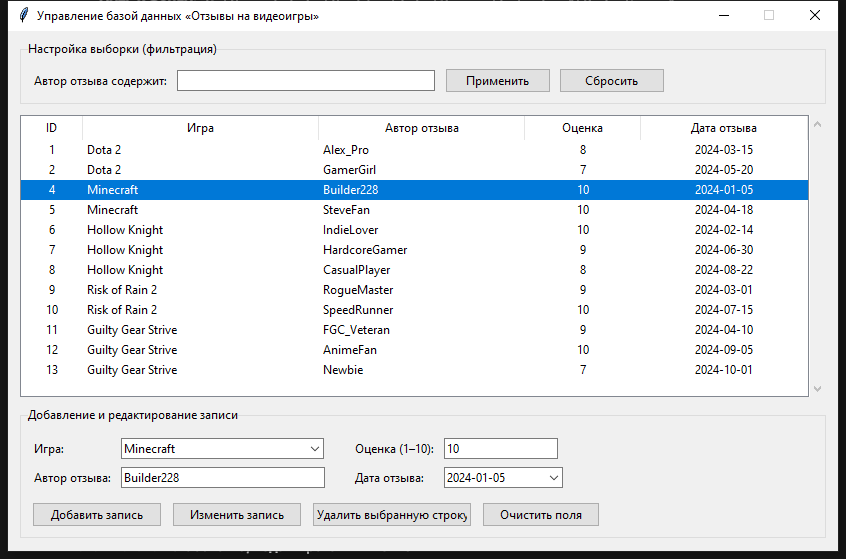
\includegraphics{s1.png}}
		\caption{Главная экранная форма приложения с загруженными данными}
	\end{figure}
	
	Выбор даты отзыва с использованием выпадающего календаря \texttt{DateEntry} представлен на рисунке~3.
	
	\begin{figure}[H]
		\centering
		\adjustbox{max width=0.92\linewidth}{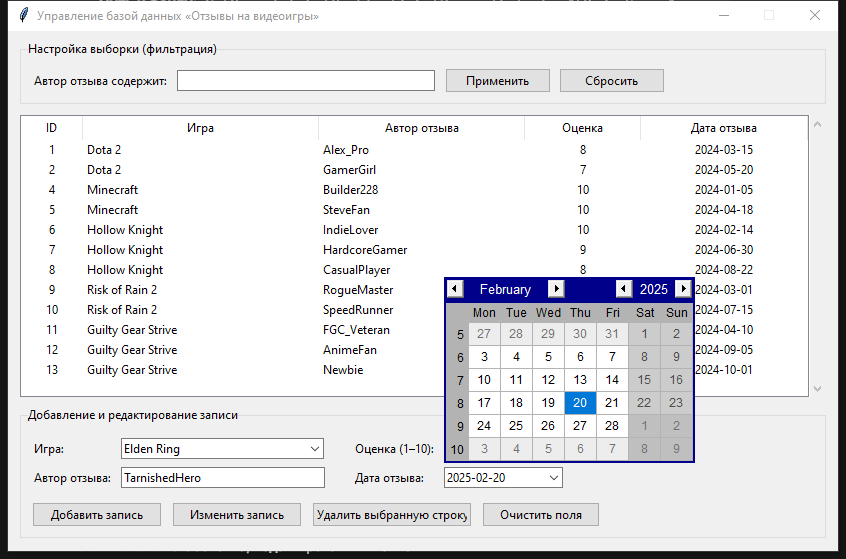
\includegraphics{s8.png}}
		\caption{Выбор даты отзыва с помощью виджета календаря}
	\end{figure}
	
	Результат добавления новой записи в таблицу \texttt{review} с помощью PL/pgSQL-функции \texttt{lab\_schema.save\_review} показан на рисунке~4.
	
	\begin{figure}[H]
		\centering
		\adjustbox{max width=0.92\linewidth}{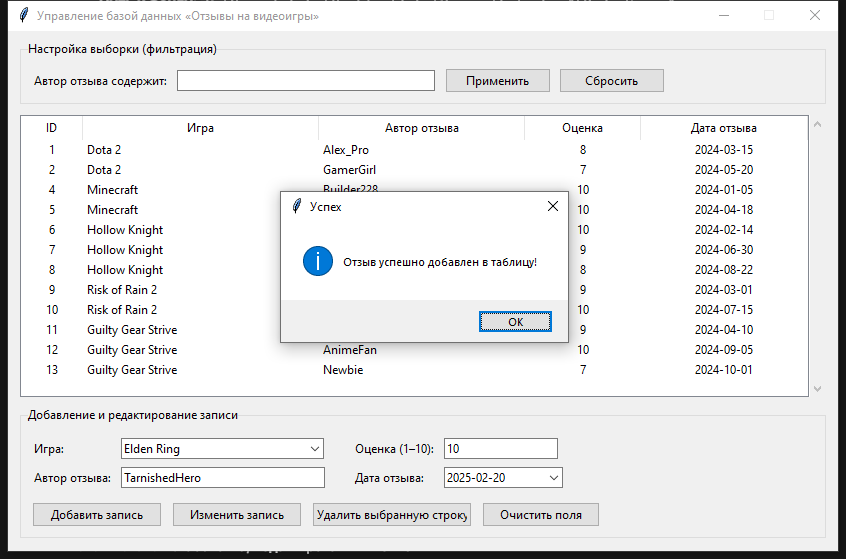
\includegraphics{s2.png}}
		\caption{Добавление новой записи в таблицу}
	\end{figure}
	
	При попытке повторного ввода уже существующих данных пользователю выводится предупреждающее сообщение без записи дубликата в таблицу (рисунок~5).
	
	\begin{figure}[H]
		\centering
		\adjustbox{max width=0.92\linewidth}{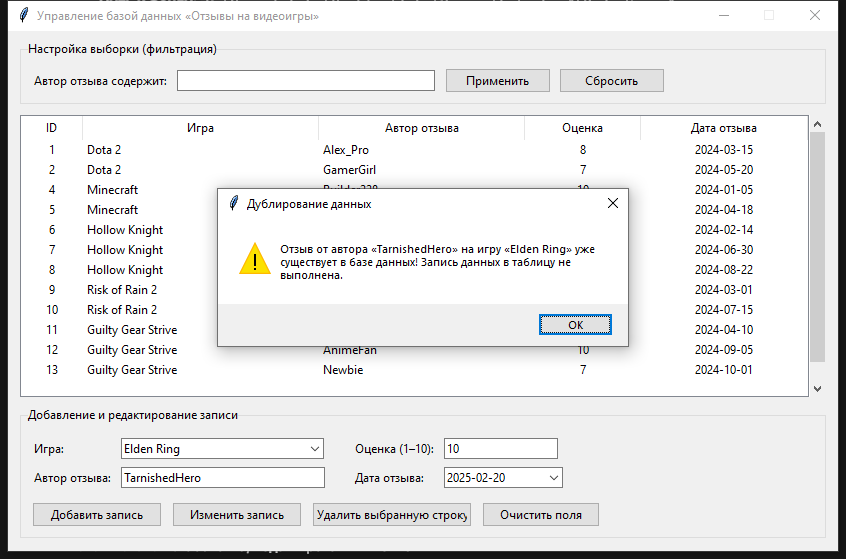
\includegraphics{s3.png}}
		\caption{Сообщение при попытке ввода уже имеющихся данных}
	\end{figure}
	
	Проверка запрета ввода отрицательных значений для числового поля «Оценка» представлена на рисунке~6.
	
	\begin{figure}[H]
		\centering
		\adjustbox{max width=0.92\linewidth}{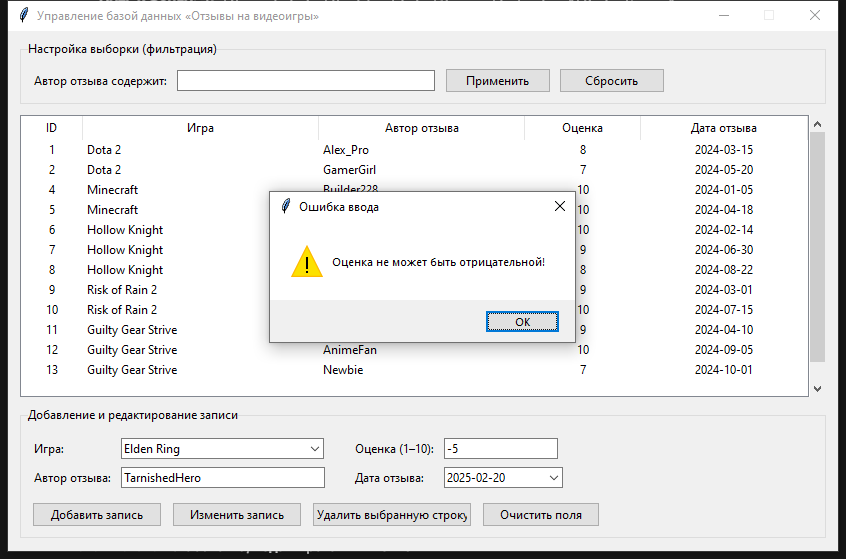
\includegraphics{s4.png}}
		\caption{Запрет ввода отрицательного значения оценки}
	\end{figure}
	
	Результат изменения существующей записи таблицы с помощью функции \texttt{lab\_schema.save\_review} показан на рисунке~7.
	
	\begin{figure}[H]
		\centering
		\adjustbox{max width=0.92\linewidth}{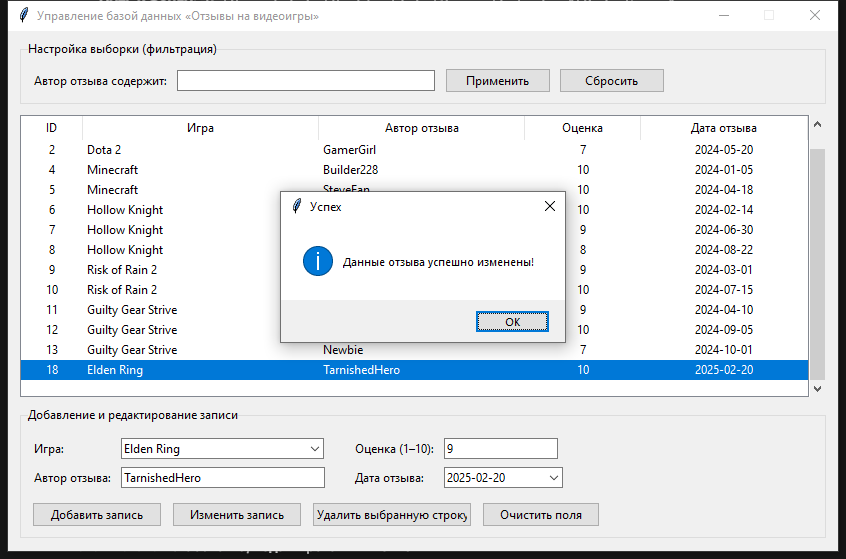
\includegraphics{s5.png}}
		\caption{Изменение данных выбранной записи}
	\end{figure}
	
	Работа регистронезависимого фильтра по строковому значению (ввод подстроки \texttt{indie} в нижнем регистре находит автора \texttt{IndieLover} через SQL-запрос с использованием функции \texttt{UPPER}) представлена на рисунке~8.
	
	\begin{figure}[H]
		\centering
		\adjustbox{max width=0.92\linewidth}{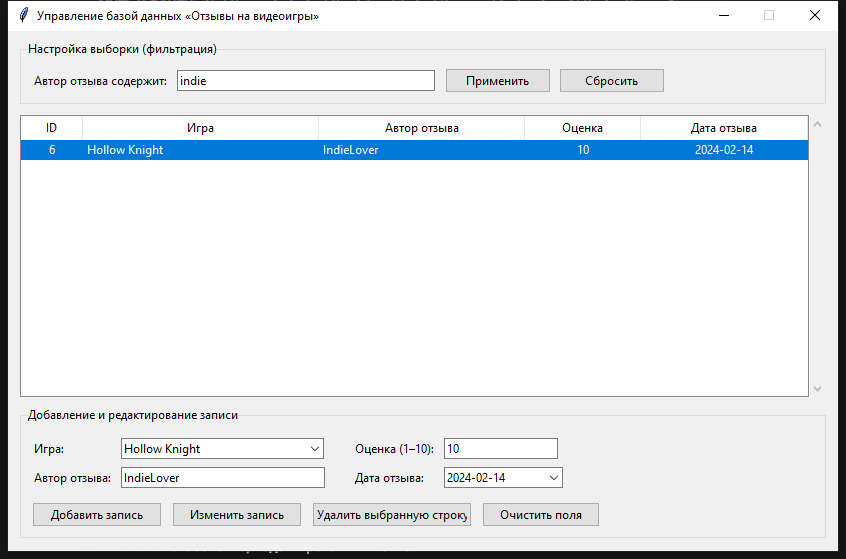
\includegraphics{s6.png}}
		\caption{Регистронезависимая фильтрация записей через запрос к БД}
	\end{figure}
	
	Диалоговое окно подтверждения удаления выбранной строки («Вы действительно уверены, что хотите удалить выбранную запись?» Да/Нет) перед вызовом PL/pgSQL-функции \texttt{lab\_schema.delete\_review} показано на рисунке~9.
	
	\begin{figure}[H]
		\centering
		\adjustbox{max width=0.92\linewidth}{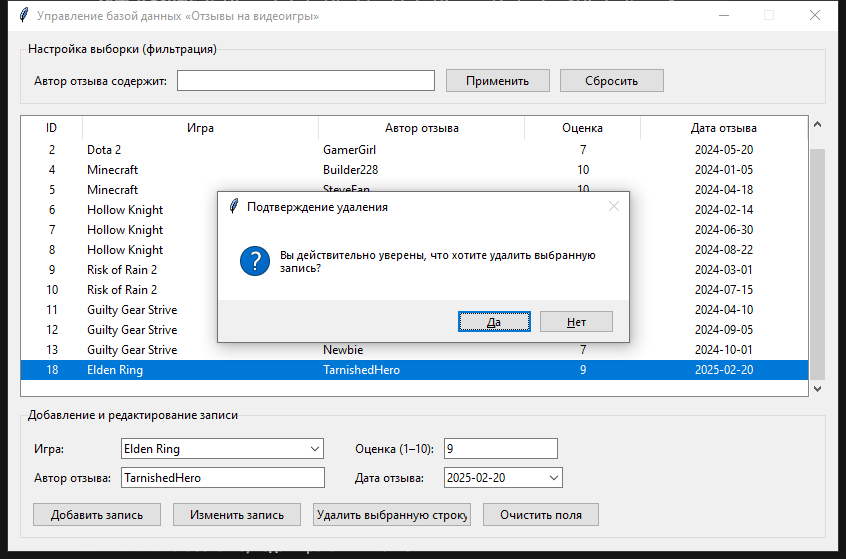
\includegraphics{s7.png}}
		\caption{Подтверждение удаления выбранной записи}
	\end{figure}
	
	\newpage
	
	\section*{Выводы} В ходе выполнения лабораторной работы были изучены средства языка Python для взаимодействия с базой данных под управлением СУБД PostgreSQL. Разработан модуль \texttt{database.py} для управления подключением и транзакциями, а также спроектирована архитектура приложения на основе шаблона проектирования Repository (DAO) и составлена диаграмма классов. Создано приложение с русскоязычным графическим интерфейсом на базе библиотеки Tkinter и виджета календаря \texttt{tkcalendar.DateEntry} для работы с таблицей \texttt{review}, ссылающейся по внешнему ключу на таблицу \texttt{game}. Реализованы вывод, добавление, редактирование и удаление записей с подтверждением через функции PL/pgSQL, выбор внешнего ключа из списка названий родительской таблицы, ввод даты через календарь, запрет ввода отрицательных значений, защита от дублирования данных и регистронезависимая фильтрация через SQL-запрос с использованием функции \texttt{UPPER}.
	
\end{document}
